\documentclass[a4paper]{report}
\usepackage{a4wide}
\usepackage[utf8]{inputenc}
\usepackage{parskip}
\usepackage{hyperref}
\usepackage{epsfig}
\usepackage{background}
\usepackage{mathptmx}

% To avoid tikz error, see https://tex.stackexchange.com/questions/165929/semiverbatim-with-tikz-in-beamer
\makeatletter
\global\let\tikz@ensure@dollar@catcode=\relax
\makeatother

\backgroundsetup{
scale=1,
angle=0,
opacity=1,
contents={
\includegraphics[width=\paperwidth,height=\paperheight]{images/spi-front.jpg}}
}

\hypersetup{
  colorlinks   = true,
  urlcolor     = blue,
  linkcolor    = blue,
  pdfinfo = {
    Title = {SPI Annual Report 2018},
    Author = {Software in the Public Interest, Inc.},
    Keywords = {SPI, free software, open source, FOSS, annual report, charity, non-profit, 501c3},
  }
}

\begin{document}

\title{Software in the Public Interest, Inc.\\
2018 Annual Report}
\date{March 11, 2019}

\maketitle

\newpage

\backgroundsetup{
scale=1,
angle=0,
opacity=1,
contents={
\includegraphics[width=\paperwidth,height=\paperheight]{images/spi-content.jpg}}
}

\hspace{1em}

To the membership, board and friends of Software in the Public Interest, Inc:

As mandated by Article 8 of the SPI Bylaws, I respectfully submit this annual
report on the activities of Software in the Public Interest, Inc. and extend my
thanks to all of those who contributed to the mission of SPI in the past year.

  \emph{-- Jimmy Kaplowitz, SPI President}

\newpage

\tableofcontents

\newpage

\chapter{President's Welcome}
\label{sec:president}

SPI serves the free software and open source community by facilitating the
administrative and financial needs of its associated projects.

During the current board term SPI continues to strive for self-improvement and
renewal. Treasury team sprints, bank visits, and legal consultations during
in-person meetings have helped keep the wheels turning. An overhaul of our
corporate bylaws that better meets our needs is being presented to the members
for their approval. And we have improved our reimbursement workflow with a
view toward speedier and smoother processing.

Every month we welcome new associated projects to SPI, along with donations
large and small for them and for our general fund. A few projects have ceased
operating or are shifting to other organizational homes, as is normal when
needs change. But in general, our model still fills a unique niche and remains
appreciated by the community.

At the same time, our scale is growing beyond what an all-volunteer
organization can smoothly handle. We are not planning to abandon the volunteer
nature of our officer and director roles, but we are exploring both short-term
and long-term possibilities for paid help to keep SPI healthy into the future.

On a personal note, I want to highlight and thank Martin Michlmayr for his
sustained dedication to SPI, including two years as SPI President before the
current board term and service as SPI Secretary before that. He remains a
valuable asset to SPI as a director, a treasury team volunteer, and possibly
in other roles as well going forward.

Thanks very much as well to all our officers, directors, volunteers, and
members for your contributions! We wouldn't be here without you.

  \emph{-- Jimmy Kaplowitz, SPI President}

\chapter{Committee Reports}
\section{Membership Committee}

\subsection{Statistics}

On January 1, 2018 we had 255 contributing and 960 non-contributing
members.  On December 31, 2018 there were 212 contributing members and
1082 non-contributing members.

\subsection{Active membership clean up}

After the 2018 board election the membership committee performed an
activity ping on members who didn't vote, as per
\href{https://spi-inc.org/corporate/resolutions/2009/2009-11-04.jmd.1/}{resolution
2009-11-04.jmd.1}, in order to determine inactive contributing members.
As a result of this, 55 inactive contributing members were moved to the
non-contributing members category.

\chapter{Board Report}
\section{Board Members}

Board members as of January 1, 2018:

\begin{itemize}
\item Martin Michlmayr (President)
\item Luca Filipozzi (Vice President)
\item Valerie Young (Secretary)
\item Michael Schultheiss (Treasurer)
\item Joerg Jaspert
\item Jimmy Kaplowitz
\item Tim Potter
\item Andrew Tridgell
\item Martin Zobel-Helas
\end{itemize}

Board members as of December 31, 2018:

\begin{itemize}
\item Jimmy Kaplowitz (President)
\item Luca Filipozzi (Vice President)
\item Tim Potter (Secretary)
\item Michael Schultheiss (Treasurer)
\item Stephen Frost
\item Dimitri John Ledkov
\item Martin Michlmayr
\item Andrew Tridgell
\item Martin Zobel-Helas
\end{itemize}

Advisors to the board as of December 31, 2018:

\begin{itemize}
\item Software Freedom Law Center (SFLC), legal counsel
\item Chris Lamb, Debian Project representative
\item Robert Treat, PostgreSQL Project representative
\end{itemize}

\section{Board Changes}

Changes that occurred during the year:

\begin{itemize}

\item Joerg Jaspert resigned from the board in February 2018 due to
lack of time.  We'd like to thank Joerg for his contributions!

\item The board appointed R. Tyler Croy as an interim director in March
2018.

\item Luca Filipozzi generously offered to resign early to reset the
election of board members to three per year. SPI typically elects three
(out of nine) board members each year but this got out of sync over the
years.

\item The terms for R. Tyler Croy and Michael Schultheiss expired in
July 2018.

\item Croy, Filipozzi and Schultheiss sought re-election.  Filipozzi and
Schultheiss were re-elected.  Stephen Frost joined the board as part of
the same election.

\item On August 13, 2018 the board voted to appoint the following
officers:

\begin{itemize}
\item President: Jimmy Kaplowitz
\item Vice President: Luca Filipozzi
\item Secretary: Tim Potter
\item Treasurer: Michael Schultheiss
\end{itemize}

\item Valerie Young resigned from the board in September 2018 due to
lack of time.  We'd like to thank Valerie for her contributions!

\item The board appointed Dimitri John Ledkov as an interim director
in September 2018.

\end{itemize}

\section{Elections}

A board membership election was conducted in July 2018.  There were 3
board seats up for election.  Nominations were received from R. Tyler
Croy, Luca Filipozzi, Stephen Frost, and Michael Schultheiss.  Luca
Filipozzi, Stephen Frost, and Michael Schultheiss were elected for a 3
year term.

\section{Face-to-face Meetings}

The SPI board held a face-to-face meeting on October 5-6, 2018.
The meeting was kindly hosted by Hudson River Trading in New York.

We discussed many topics, including treasurer activities, IT
infrastructure, the need for various policies, and more paid help for
SPI's operations.

We also held a treasurer sprint immediately before the board meeting.
The venue for the sprint was provided by Crunchy Data.

\begin{figure*}[h]
\centering

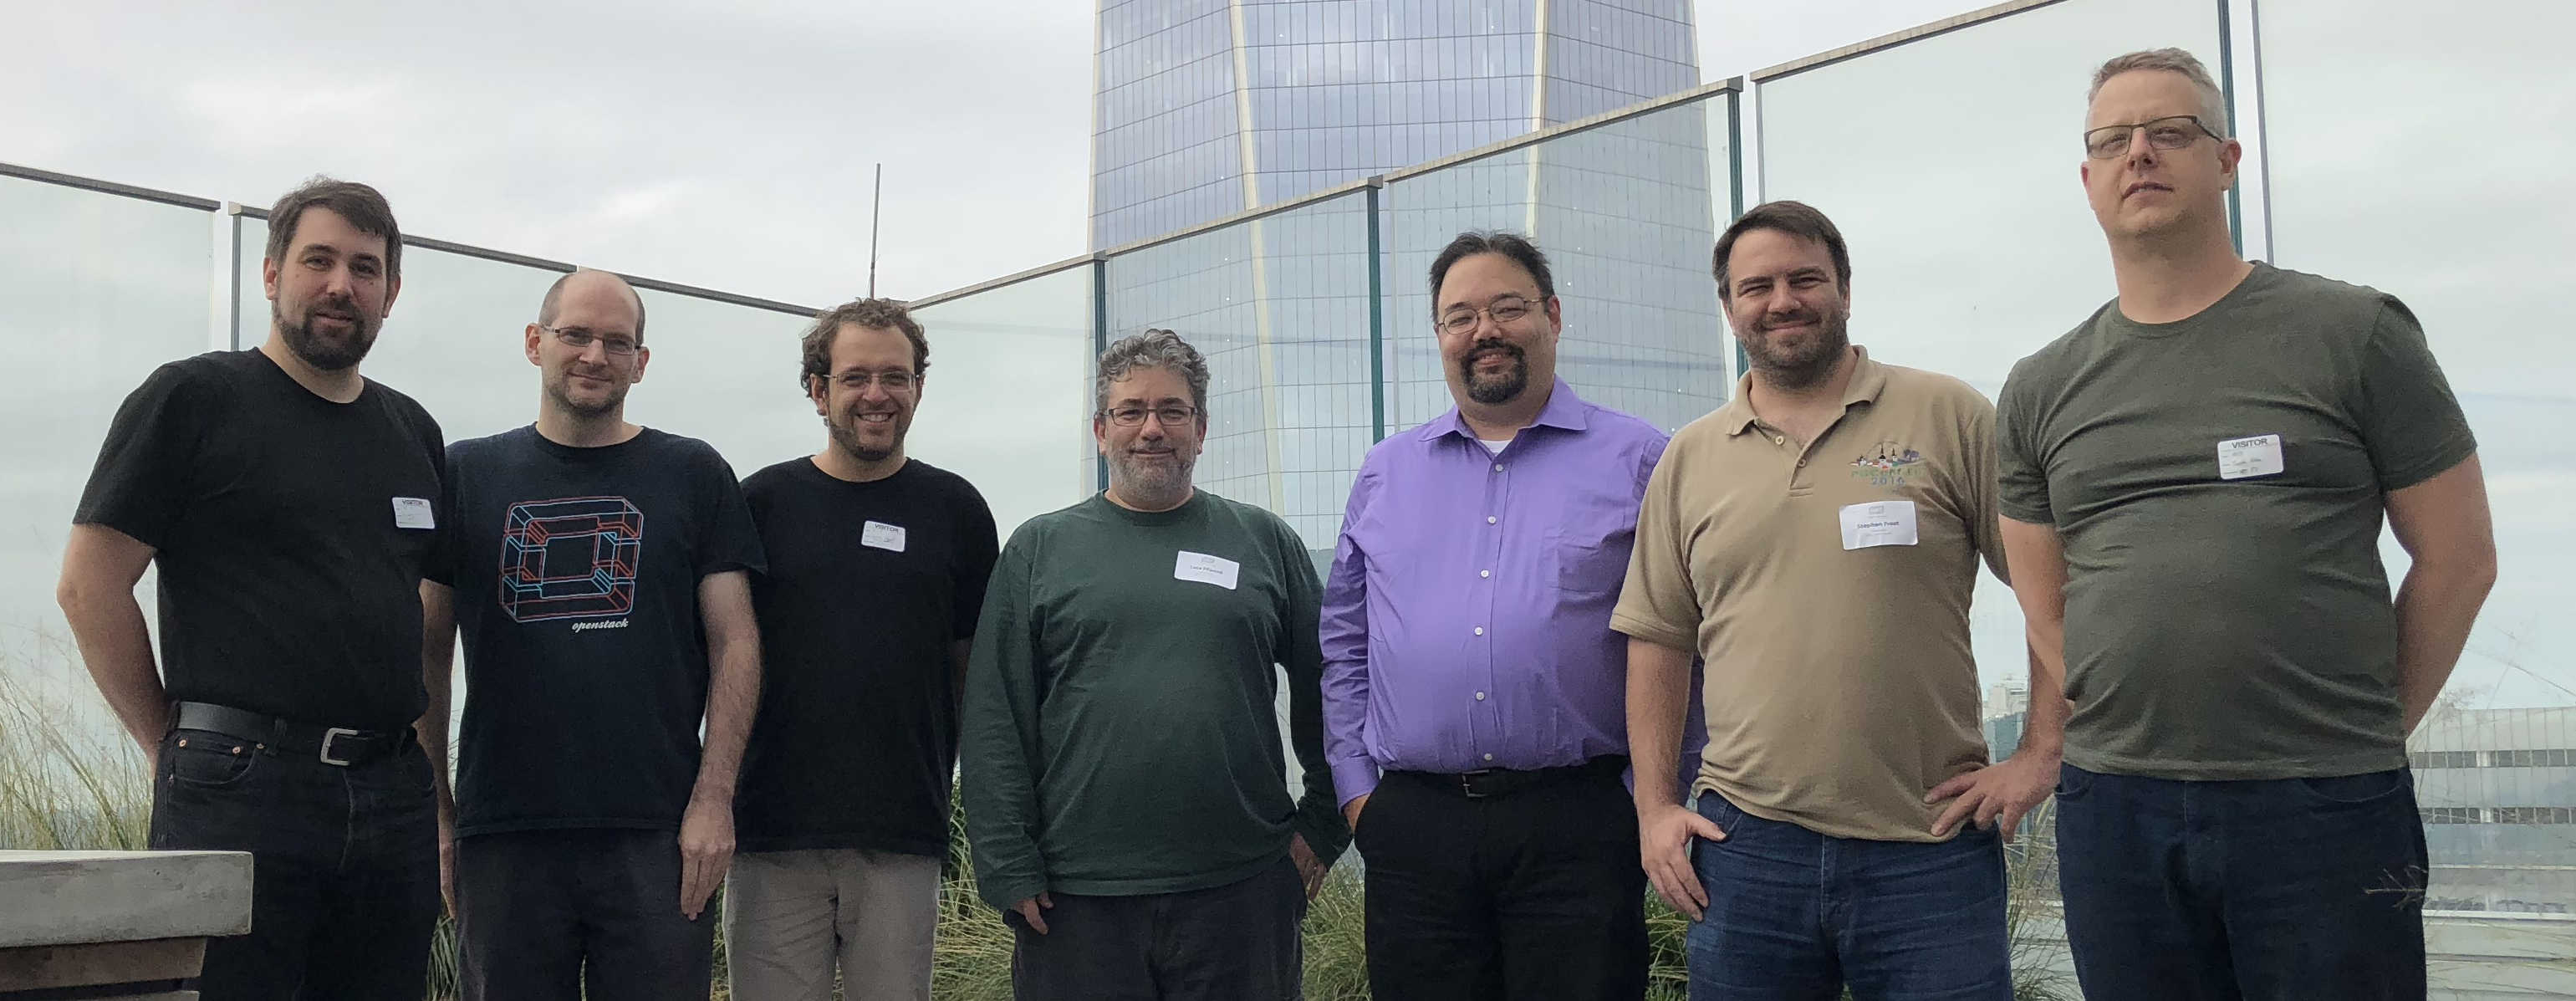
\includegraphics[scale=0.14]{images/2018-october-f2f}

\caption{Face-to-face meeting in New York (October 2018): Martin
Zobel-Helas, Martin Michlmayr, Jimmy Kaplowitz, Luca Filipozzi, Michael
Schultheiss, Stephen Frost, and Tim Potter (left to right)}

\end{figure*}

\chapter{Treasury Report}

This report uses a cash-based method of accounting, recording donations
when deposited (not when the check was written or received by us) and
recording expenses when sent or scheduled for payment (not when
incurred).

{\em These figures are provisional and subject to change.}

\section{Income Statement}

This covers the Period January 1, 2018 -- December 31, 2018

\begin{verbatim}
 Income
   Ordinary Income
        0 A.D.                           3,190.54
        Ankur                                0.00
        Aptosid                            147.70
        Arch Linux                     294,268.56
        ArduPilot                       40,465.51
        Chakra                             388.34
        DebConf                         18,654.20
        DebConf17                        9,975.00
        DebConf18                      116,635.08
        DebConf19                        4,750.00
        Debian                         337,196.28
        Drizzle                              0.00
        FFmpeg                         105,606.05
        FFmpeg (OPW)                     1,140.00
        Fluxbox                              1.15
        freedesktop.org                    203.78
        Gallery                              0.00
        Glucosio                             3.42
        GNU TeXmacs                        161.50
        GNUstep                              0.00
        haskell.org                         57.00
        Jenkins                          6,202.25
        LibreOffice                     16,786.97
        MadWifi                         (1,494.90)
        MinGW                               29.90
        NTPsec                             674.54
        Open Bioinformatics              5,451.18
        Open MPI                            95.00
        Open Voting Foundation              29.00
        OpenEmbedded                       313.79
        OpenVAS                              9.50
        OpenWrt                          2,368.48
        OpenZFS                         22,168.48
        OSUNIX                             (17.17)
        Path64                             (18.60)
        Performance Co-Pilot             4,940.00
        PostgreSQL                      30,961.05
        Privoxy                              1.04
        Swathanthra Malayalam Computing      0.00
        SPI General                    205,298.29
        systemd                        190,004.75
        The HeliOS Project                   0.00
        Torch                                1.47
        Tux4Kids                           (19.00)
        X.Org                           39,981.73
        YafaRay                              0.00

        Total Ordinary Income        1,456,257.87
                                     ------------
   Interest Income
        Ameriprise Brokerage                54.48
        Key Business Platinum MM Savings    89.03
        Chase BusSelect High Yield Savings 108.33
        Fifth Third Business MM 128         14.96

        Total Interest Income              266.80
                                           ------

   Gross Income                      1,456,524.67
                                     ------------

 Expenses
  Ordinary Expenses

        0 A.D.
          182.84    Banking fees
        1,283.34    IT
          576.97    Meetups
        --------
        2,043.15

        Ankur
            0.00

        Aptosid
            6.17    Banking fees

        Arch Linux
          492.94    Banking fees
        4,191.95    IT
        --------
        4,684.89

        ArduPilot
        1,252.28    Banking fees
       24,482.40    Development
        6,916.33    IT
        8,856.31    Meetups
       ---------
       41,507.32

        Chakra
            8.89    Banking fees
          681.72    IT
          ------
          690.61

        DebConf
          848.05    Banking fees

        DebConf 17
           92.05    Banking fees
       12,037.01    Meetups
       ---------
       12,129.06

        DebConf 18
           50.88    Banking fees
          608.53    IT
      112,653.01    Meetups
      ----------
      113,312.42

        DebConf 19
        4,083.53    Meetups

        Debian
        1,565.78    Banking fees
       19,500.00    Development
       27,326.93    IT
       23,764.93    Meetups
        6,323.12    Office
       ---------
       78,480.76

        Drizzle
            0.00

        FFmpeg
          213.47    Banking fees
        5,430.60    Development
        2,418.69    Meetups
        --------
        8,062.76

        FFmpeg (OPW)
            51.15   Banking fees

        Fluxbox
            0.33    Banking fees

        freedesktop.org
            9.79    Banking fees
        1,500.00    Development
        7,384.60    IT
        ---------
        8,894.39

        Gallery
            0.00

        Glucosio
            1.58    Banking fees

        GNU TeXmacs
            7.59    Banking fees

        haskell.org
             2.75   Banking fees

        Jenkins
           78.49    Banking fees
          300.00    IT
        3,589.78    Meetups
         -------
        3,968.27

        LibreOffice
          213.52    Banking fees
       32,041.54    Meetups
       ---------
       32,255.06

        MinGW
            2.23    Banking fees

        NTPsec
           28.16    Banking fees
        6,100.00    Development
        --------
        6,128.16

        Open Bioinformatics
            0.87    Banking fees
        3,961.67    IT
          906.00    Meetups
        --------
        4,868.54

        OpenEmbedded
           17.51    Banking fees

        Open MPI
            4.35    Banking fees

        Open Voting Foundation
            1.45    Banking fees

        OpenVAS
            1.05    Banking fees

        OpenWrt
           39.49    Banking fees

        OpenZFS
          355.92    Banking fees
        1,289.46    IT
       19,324.27    Meetups
          359.90    Office
       ---------
       21,329.55

        Performance Co-Pilot
            0.30    Banking fees
          681.22    Development
        4,493.73    Meetups
        --------
        5,175.25

        PostgreSQL
           33.68    Banking fees
        1,082.79    Development
          774.00    Meetups
        --------
        1,890.47

        privoxy
            0.32    Banking fees

        Swathanthra Malayalam Computing
            0.00

        SPI
        1,162.14    Banking fees
       15,681.81    Meetups
        4,303.68    Office
       ---------
       21,147.63

        systemd
            0.55    Banking fees

        Torch
            0.63    Banking fees

        Tux4Kids
           (0.44)   Banking fees

        X.Org
          682.54    Banking fees
        2,774.03    Development
        8,868.02    Meetups
           25.00    Office
       ---------
       12,349.59

        YafaRay
          746.37    IT

        Total Expenses          384,732.54
                                ----------

        Net Income            1,071,792.13
\end{verbatim}

\section{Balance Sheet}

\begin{verbatim}
Balance Sheet as of December 31, 2018

   ASSETS
     Current Assets
        Ameriprise Cash Mgmt Acct                         13,498.19
        Bank of America Business Advantage Checking      250,000.00
        Chase Business Select High Yield Savings          55,333.94
        Chase Performance Business Checking              101,078.17
        Fifth Third Business Elite Checking (Debian)     131,899.39
        Fifth Third Business Elite Checking (SPI)         91,569.24
        Fifth Third Business Elite Checking Wiretransfer 164,060.11
        Fifth Third Business Money Market 128             30,019.88
        KeyBank Basic Business Checking                    8,919.08
        Key Business Platinum Money Market Savings     1,000,066.46
        Key Business Reward Checking                     301,857.93
        PayPal (Debian)                                    3,400.73
        PayPal (SPI)                                       3,331.07

     Total Current Assets                              2,155,034.19

   TOTAL ASSETS                                        2,155,034.19

   LIABILITIES AND EQUITY

     General and current liabilities                           0.00

     Equity
        Reserves held in trust
           0 A.D.                            32,430.79
           ankur.org.in                       2,819.84
           aptosid                              485.50
           Arch Linux                       337,213.85
           ArduPilot                         63,797.78
           Chakra                               553.85
           DebConf                           17,806.15
           DebConf 14                        35,962.78
           DebConf 15                        70,218.51
           DebConf 16                       (15,395.06)
           DebConf 17                       (17,163.37)
           DebConf 18                         3,322.66
           DebConf 19                           666.47
           Debian                           463,443.61
           Drizzle                            6,148.60
           FFmpeg                           113,443.53
           FFmpeg (Outreachy)                 1,737.38
           Fluxbox                              997.96
           freedesktop.org                    6,575.52
           FreedomBox Foundation                 23.52
           Gallery                                0.00
           Glucosio                               1.84
           GNU TeXmacs                        1,300.86
           GNUstep                              142.50
           Haskell                           16,537.14
           Jenkins                           31,906.58
           LibreOffice                       31,508.76
           MadWifi                                0.00
           MinGW                              4,160.53
           NTPsec                               631.67
           Open Bioinformatics               84,508.17
           Open MPI                             636.90
           Open Voting Foundation               144.27
           OpenEmbedded                         732.07
           OpenVAS                               73.49
           OpenWrt                            8,662.19
           OpenZFS                              583.44
           OSUNIX                                 0.00
           Path64                                 0.00
           Performance Co-Pilot               5,353.20
           PostgreSQL                       148,292.82
           Privoxy                            1,735.96
           Swathanthra Malayan Comp           5,763.32
           systemd                          190,004.20
           The HeliOS Project                   212.83
           TideSDK                                0.00
           Torch                                  0.84
           Tux4Kids                          16,284.59
           X.Org                             66,298.49
           YafaRay                            6,229.96

        Total held in trust                            1,746,796.49

        General reserves                                 408,237.70

     Total Equity                                      2,155,034.19

   TOTAL LIABILITIES AND EQUITY                        2,155,034.19
\end{verbatim}

\chapter{Member Project Reports}

\section{New Associated Projects}

In 2018, systemd joined the SPI umbrella as an associated project.

\subsection{systemd}

systemd is a suite of basic building blocks for a Linux system. It
provides a system and service manager that runs as PID 1 and starts the
rest of the system. systemd provides aggressive parallelization
capabilities, uses socket and D-Bus activation for starting services,
offers on-demand starting of daemons, keeps track of processes using
Linux control groups, maintains mount and automount points, and
implements elaborate transactional dependency-based service control logic.

\section{Projects No Longer Associated with SPI}

\begin{itemize}

\item Fresco (originally named the Berlin Project) was a windowing
system derived from a powerful structured graphics toolkit
originally based on InterViews.  The project hasn't been active
for many years.

\item MadWifi was a project to coordinate development of the Atheros
drivers for Linux.  The MadWifi driver has been obsoleted by
{\tt ath5k} and {\tt ath9k}, which are both part of the Linux kernel
now.

\item Open64 is an open source compiler based on Pro64.  SPI has not
provided any services to Open64 in several years.

\item OSUNIX was an open source OpenSolaris technology distribution.
The project is no longer active.

\item Path64 was the open source community version of PathScale's
compiler.  The project is no longer active.

\item TideSDK was an HTML5, CSS3 and JavaScript framework.  The
project is no longer active.

\item The HeliOS Project rescued computers and refurbished them and
gave them to disadvantaged children in Central Texas.  The HeliOS
Project no longer exists as a standalone project and its activities
have been taken on by the Reglue project.

\end{itemize}

\section{Updates from Associated Projects}

\subsection{0 A.D.}

0 A.D. (pronounced ``zero ey-dee'') is a cross-platform, real-time
strategy (RTS) game of ancient warfare. It is a historically-based
war/economy game, in which the player must lead an ancient civilization,
gather resources from the map, and raise a military force to conquer
enemy factions. 0 A.D. is open source software licensed under the GPL,
and its art and sound assets are licensed under CC BY-SA. It is
developed by Wildfire Games, a global community of game developers.

In mid-2018, we released Alpha 23 Ken Wood, available for Windows,
macOS, and Linux, named in memory of one of the original gameplay
designers of 0 A.D. This alpha version introduced a new faction, the
Kushites, several new maps, and many improvements to the gameplay, the
user interface, the artwork, the security of the multiplayer mode, and
more.  Importantly, this new version also came with a mod downloader,
which allows users to download and install mods without leaving the
game. This is achieved using mod.io, a new and powerful cross-platform
modding API.  0 A.D. was one of the few inaugural game titles to support
this innovative modding solution with its launch.

A few months after the release of Alpha 23 Ken Wood, we issued an
additional minor release to fix several critical bugs and to address
important security and legal issues, including GDPR compliance.

According to our records, Alpha 23 Ken Wood was downloaded over 110,000
times in 2018. (That figure is a conservative estimate, as it does not
include downloads performed through the Linux distributions' package
managers.) Additionally, the in-game mod installer was used tens of
thousands of times in 2018.

The 0 A.D. soundtrack became available on several music streaming
services (Spotify, Amazon, Google Play Music, iTunes, and Deezer). This
was accomplished through Materia Collective, a video game soundtrack
record label and music publisher.

Last but not least, members of Wildfire Games attended two FOSS
community events in 2018, and presented the game to the attendees:
FOSDEM (Brussels, Belgium) and LDLL (Lyon, France). This helped raise
awareness of 0 A.D. and facilitated recruitment of developers.

We wish to extend our thanks to our generous donors and to SPI for
helping us achieve this progress.

\subsection{ArduPilot}

ArduPilot is a cross-platform free software autopilot project for all
types of small robotic vehicles.  ArduPilot continues to thrive, with a
global and growing community of users, partners and developers.
Significant effort over the past year has seen a successful transition
to the ChibiOS RTOS, and the addition of a new generation of micro
controller to the standard builds (ARM Cortex M7).  Many new features
have been added, with new vehicle types (such as Balance Bots,
Sailboats, and complex Hybrid VTOL Airplanes), new sensors, and
increased support for ROS (Robot Operating System) interaction.  The
2018 Developers Conference was a great success, with the 2019 Conference
promising to build upon it, and be the largest conglomeration of
ArduPilot developers yet.

{\em Submitted by James Pattison}

\subsection{Chakra}

Chakra is a GNU/Linux distribution with an emphasis on KDE and Qt
technologies that focuses on simplicity from a technical standpoint and
free software.

In February, we carried out rebuilds for the GCC ABI changes. In April,
Pacman 5 with its new features such as hooks and file database
operations was made available to our users. In July, we received a
sponsorship by GitLab Inc., giving us access to all the features of the
enterprise edition of their software. In December, Linux 4.19 with the
patch set by Con Kolivas was made available to our testers. These are
patches designed to improve system responsiveness and interactivity with
specific emphasis on the desktop, but configurable for any workload.
Finally, Chakra has now been registered as a group on the Freenode
network. This represents an official relationship between Chakra and
Freenode, and indicates that we are maintaining an official presence on
their network.

{\em Submitted by Hans Tovetjärn}

\subsection{Debian}

The next stable release of the Debian distribution (``buster'') has been
taking shape throughout 2018 and we tentatively plan to release in Q2 in
2019.

In addition, the large migration to a new hosting infrastructure
platform (based on the GitLab platform) was completed with many tangible
improvements to workflows, etc.  Debian's ``DebConf'' annual gathering
was successfully held in Hsinchu, Taiwan too.

On Thursday 16th August 2018 the Debian project celebrated its
\href{https://bits.debian.org/2018/08/debian-is-25.html}{25th
anniversary}.  This is a new milestone for the project and makes it one
of the oldest Free and Open Source GNU/Linux distributions.

{\em Submitted by Chris Lamb, Debian Project Leader}

\subsection{Drizzle}

The Drizzle database server is no longer actively developed.  However,
two of the client libraries are still in active use and development:
drizzle-jdbc (Java) and libdrizzle-redux (C).  One motivation for
continued use of these libraries is that they provide permissively
licensed client libraries compatible with the MySQL protocol.

{\em Submitted by Henrik Ingo}

\subsection{FFmpeg}

FFmpeg is a complete, cross-platform solution to record, convert and
stream audio and video. It is used as the platform foundation of many
projects dealing with multimedia, both open source and proprietary, and
used extensively by several multimedia web-based multimedia conversion
and processing services.

In the year 2018 FFmpeg delivered two formal releases (4.0 and 4.1) and
several security updates of old releases. A complete list of changes can
be \href{https://git.ffmpeg.org/gitweb/ffmpeg.git/blob/HEAD:/Changelog}{found
in the changelog}.  Also, as usual, FFmpeg joined the GSoC program, with
total of 5 assigned projects.

FFmpeg attended various conferences and meetups during the year.
Several developers attended to represent and connect the project with
our users and fellow open source projects.  These include venues in
Europe and abroad, covering pure end-user conferences, developer meetups
of fellow projects to the annual summit of GSoC affiliate program.
FFmpeg ordered various merchandise stock to give away during these
attendances. Also, some promotional items are kept in stock and extended
for necessities depending on the corresponding venue.

{\em Submitted by Stefano Sabatini and Thilo Borgmann}

\subsection{GNU TeXmacs}

GNU TeXmacs is a free scientific office suite with a professional
typesetting quality.  Our focus in 2018 has been on the preparation of a
new major version that we plan to release during 2019.  As a
consequence, we have fixed many bugs, improved the robustness of TeXmacs
on the platforms that we support, and started the generation of our own
packages for various GNU/Linux distributions.

{\em Submitted by Joris van der Hoeven}

\subsection{Jenkins}

Jenkins continues to play a major role in pushing the automation
forward, after 14+ years since its birth, and if anything the pace of
growth seems to be accelerating. In this dog year industry, that's truly
remarkable. Being a part of this achievement truly makes me proud. That
faster pace results in what I call ``5 super powers'':

\begin{itemize}

\item \href{https://jenkins-x.io/}{Jenkins X} is probably the most
visible innovation of this year, making it much easier to create modern
cloud applications on Kubernetes. This also represents the significant
expansion of the
\href{https://jenkins.io/blog/2018/03/20/evolving-mission-of-jenkins/}{Jenkins
community and its mission}.

\item \href{https://jenkins.io/projects/jcasc/}{Jenkins Configuration as
Code} hit a major milestone 1.0 this year, and it's continuing to gain
more momentum and traction.

\item ``Cloud Native Jenkins'' is the term I gave to a new effort that
I'm calling to transform Jenkins into a general purpose CI/CD engine that
runs at scale on Kubernetes. There's still much to be defined here, but
you can already see some great things like Serverless Jenkins.

\item \href{https://jenkins.io/projects/evergreen/}{Evergreen} is another
young and upcoming project that has an ambitious thesis --- drastically
simplifying the adoption and operation of Jenkins.

\item Pipeline effort formed a new SIG and I'm looking forward to the
impact this will drive in 2019.

\end{itemize}

The not-so-secret sauce of the Jenkins community that threads together
all these improvements from user visible changes to the community
improvements is our ability to evolve. As I look forward to 2019, no
doubt these things I mentioned will evolve, morph, merge, and split as
we continue to learn and adopt.

{\em Submitted by Kohsuke Kawaguchi}

\subsection{MinGW}

In 2018, the focus of MinGW has been on updating our core tools to the
latest upstream versions, and in the migration of file release hosting
from SourceForge.net to OSDN.net.  While older releases will remain on
SourceForge.net, the latest are distributed exclusively via OSDN.net

To accompany these updates, originating upstream, our own supporting
MinGW Windows System Libraries (comprising \texttt{mingwrt} and
\texttt{w32api}), have been updated to version 5.2 (with a critical
5.2.1 patch release, in January 2019).

{\em Submitted by Keith Marshall}

\subsection{LibreOffice}

In 2018, the LibreOffice project released two new versions of the
software (6.0 and 6.1) along with several smaller bug fix updates.
LibreOffice 6.0 introduced an ePUB export filter for saving documents as
eBooks, along with experimental document signing with OpenPGP.
Meanwhile, LibreOffice 6.1 introduced new icon themes, a revamped image
handling engine, and parallel formula compiling in the spreadsheet for
improved performance.

Throughout the year, the community organized events, such as the
LibreOffice Conference in Tirana, Albania, which took place in
September. There were also hackfests in Hamburg and Munich, bringing
developers together, while local communities organized translation
sprints, bug hunting sessions and other meetups in Japan, Nepal, Taiwan,
Turkey and other locations.

{\em Submitted by Sophie Gautier}

\subsection{NTPsec}

NTPsec continues to progress from our 1.0.0 release in late 2016.  We
are now at version 1.1.3.  Through 2017 we continue to clean up and
refactor the codebase, and have maintained our record of immunity and
rapid fixes to CVEs discovered against NTP Classic.  We added support
for the internet draft features ``draft-ietf-ntp-mac'' and
``draft-ietf-ntp-data-minimization''.  We negotiated a grant from Cisco
to implement the new Network Time Security (NTS) specification, and
design work on NTS is ongoing right now.

{\em Submitted by Mark Atwood}

\subsection{OFTC}

OFTC has continued to operate the IRC network. We are slowly gaining
more staff, and the spam waves over the past months have not had any
impact on the generally good atmosphere among the operators.

{\em Submitted by Christoph Berg}

\subsection{Open Bioinformatics Foundation}

The Open Bioinformatics Foundation is a non-profit, volunteer-run group
dedicated to promoting the practice and philosophy of open source
software development and Open Science within the biological research
community. The OBF's most visible activities are running the annual
Bioinformatics Open Source Conference (BOSC), participating in the
Google Summer of Code program, and running the OBF Travel Fellowship
program. The Travel Fellowship program, launched in 2016, aims to
improve diversity at bioinformatics events. As of January 2019, there
have been 85 applicants over nine application rounds, and a total of
twelve fellowships were awarded. The OBF functions as a GSoC umbrella
organization for bioinformatics projects. 38 students have participated
in summer internships under the OBF umbrella since 2010.

{\em Submitted by Nomi Harris}

\subsection{OpenEmbedded}

OpenEmbedded is a build system that creates custom Linux distributions
for devices running Linux. Traditionally used for creating images for
embedded devices, OpenEmbedded is now used all over to create small
images for internet of things (IoT) devices, to large images pushing
into the desktop space.  Over the past year, we see additional users who
build edge routers for IoT applications and images to deploy in popular
containers systems.

To support the OpenEmbedded developer community, we work with the Yocto
Project to arrange developer meetings twice a year. Developer meetings
bring people together to review challenges facing the project and create
better relationships in the community. Moving forward, we are planning
to hold developer summits to improve communication of our capabilities
and new features.

{\em Submitted by Philip Balister}

\subsection{Open MPI}

The Open MPI community is a collection of academics, researchers, and
vendors who continue to develop cutting-edge technology for today’s
most-demanding High Performance Computing (HPC) environments. This
community had a busy year in 2018: we had eleven releases of our
signature project (Open MPI).  We had new minor releases of our v2.1.x
series: v2.1.3 through v2.1.5.  We also had new minor releases of our
v3.0.x series (v3.0.1 through v3.0.3), and introduced the v3.1.x series
with releases up through v3.1.3.  Our all-new v4.0.0 release in November
kicked off our v4.0.x series.  The Hardware Locality (hwloc) sub-project
also had several releases including contributions from both the overall
community and several vendors: the legacy v1.11 series had several
releases (v1.11.9 through v1.11.12), and the all-new v2.0.x series
debuted along with several followup bug-fix releases (up through
v2.0.3).

{\em Submitted by Jeff Squyres}

\subsection{Open Voting}

As in recent years, in 2018 we focused mainly on advocacy work. The open
source voting effort has faced significant opposition from existing
vendors. Despite this, we saw success inspiring San Francisco to proceed
with getting their own open source voting system built and certified.
The work is in early stages. Several people, including a project
manager, have been hired so far. The Mayor has assigned San Francisco's
Technology Director to lead the project. State money has been made
available for the project, although not yet allocated.

{\em Submitted by Alan Dechert}

\subsection{OpenZFS}

OpenZFS held its annual Developer Summit in September 2018. With around
100 attendees and 14 speakers, it was a great event for educating the
community about new features in OpenZFS, as well as for folks to
interact face to face with other developers and plan the next year’s
activities. We also started holding monthly leadership meetings (via
video conference) which accomplish similar goals but with a focus on
discussion rather than presentations.  On the development front, 2018
saw the integration of device removal, special devices for metadata,
zpool checkpoint, and sequential scrub/resilver.

{\em Submitted by Matthew Ahrens}

\subsection{Performance Co-Pilot}

2018 was another successful year for the PCP community; we ran our first
conference! It was held in Tokyo, Japan and was very well received.
Plans began immediately afterwards for next years conference, to be held
on March 1st 2019, in Melbourne, Australia.

We released a major version (4.0) update to PCP, followed by several
minor releases over the course of the year.  We added new analysis tools
(including a revived dstat utility), many new performance metrics and
significant new core functionality.

Once again we participated as a Google Summer of Code organization and
mentored six students and their projects this year.

{\em Submitted by Nathan Scott}

\subsection{PostgreSQL}

During 2018, PostgreSQL 11 was released, which added stored procedures
and improved partitioning and parallelism.  A multi-year project to add
just-in-time compilation was started that will greatly enhance the data
warehouse abilities of PostgreSQL in the coming years.

Quarterly minor releases were also produced.  The community development
process continues to flourish, with new people and companies constantly
joining.

After languishing for years, our website was finally updated with a
fresh appearance and new backend technology.  We adopted a code of
conduct in 2018, and our international event and user group activities
continued to grow.

{\em Submitted by Bruce Momjian}

\subsection{Privoxy}

In 2018 we released Privoxy 3.0.28 which scales better in multi-user
environments and brings a couple of new tuning directives.

{\em Submitted by Fabian Keil}

\subsection{SproutCore}

SproutCore is an open source framework for building fast, innovative
user experiences on the web. The main focus of the core team has been
to see how the way SproutCore uses JavaScript to realize its programming
model can be best transferred into the era of ES6 classes and modules.
It has become clear that some syntactical change is likely to be
necessary, and that any `native' version will have to wait till the
arrival of the function like \texttt{import()} because of runtime
dependencies.  SproutCore has moved to a new default theme which doesn't
require automated image slicing, making its build tools less
dependency-heavy. The documentation has been improved to reflect these
changes.

{\em Submitted by Maurits Lamers}

\subsection{Swathanthra Malayalam Computing (SMC)}

Swathanthra Malayalam Computing(SMC) works as an umbrella organization
of various free and open source language technology projects in Indian
languages. In 2018 SMC continued its active work on development,
research, standardization and technology policy ensuring digital rights
of native language users.

An SMC developer community meetup was held in April 2018. The Indic
keyboard project had a major release with bug fixes and support for
Santali in August 2018. Indic keyboard recently received a Mozilla Open
Source Support (MOSS) award. Mlmorph, a library for morphological
analysis for Malayalam, was released in December 2018. Mlphon, a
Malayalam phonetic analyzer, was also released in December 2018. A
popular input method, Swanalekha, is now available on all operating
systems and devices. SMC's 12+ Indian language fonts are actively
maintained and new font development projects are in progress. SMC is
actively involved in technology policy consultations on privacy and data
protection in India and organized public discussions on these topics.
SMC's localization team contributed to GNOME and Firefox Lite Malayalam
localization projects. We restarted the work on a Malayalam language
bibliography open data project, Grandham, this year.  Our community
members published papers and presented them at various conferences, such
as Grafematik 2018, State of the Map Asia 2018, DebUtsav 18 etc.

{\em Submitted by Anivar Aravind}

\subsection{systemd}

In 2018 we published four major releases of systemd (see
\href{https://raw.githubusercontent.com/systemd/systemd/master/NEWS}{complete
list of changes}).  We received a 200,000 US dollar donation from
Handshake.org.  At the {\em All Systems Go!} conference in Berlin, many
systemd contributors and maintainers participated in a successful
hackfest.

{\em Submitted by Lennart Poettering}

\subsection{The Mana World}

The Mana World (TMW) is an effort to create an innovative free and open
source MMORPG (massively multiplayer online role-playing game).  The
Mana World made further progress in
\href{https://gitlab.com/evol/serverdata}{backporting} more
\href{https://github.com/themanaworld/tmwa-server-data}{legacy TMW
content} to the
\href{https://gitlab.com/evol/evol-hercules}{Evol-Hercules engine},
while also adding new content and features that were not possible under
the older engine. Players can now have their own personal rowboat to
navigate on water and other means of transportation may be added in the
future. To ensure continued operation of the legacy server while the new
one is still being built, numerous security updates have been backported
to the deprecated tmwAthena engine.

{\em Submitted by Pascal Beauchamp}

\subsection{Tux4Kids}

A new released of Tux Paint, a drawing program for children, was
published in the latter half of 2018.  This release brings back
compatibility with macOS, adds 5 new localizations (Bengali, Bodo,
Dogri, Kabyle, Urdu), a set of star shapes in the shape-drawing tool,
and a color picker (eyedropper).

{\em Submitted by Bill Kendrick}

\subsection{X.Org}

The X.Org community creates a free and open accelerated graphics stack,
including major components such as the DRM kernel graphics subsystem,
Mesa 3D graphics library, Wayland compositor and the X.Org Window
System.

The Foundation supported the community through travel grants for the X
Developer Conference in La Coruña, Spain, organized by Igalia and GPUL
in September. 5 students successfully completed their
GSoC/EVoC/Outreachy internships within the X.Org community, and most
could attend XDC in Spain and present their work thanks to travel grants
from X.Org.

This year we've looked for sponsors for XDC for the first time since
years again, made possible thanks to SPI as our fiscal sponsors. This
was extremely successful and we managed to secure one Platinum, seven
Gold sponsors and two local sponsors at the Bronze level to support our
conference

The X.org board has spent a lot of time working together with the
freedesktop.org project to prepare our merger, which aims to streamline
and improve how we run both of our communities.

{\em Submitted by Daniel Vetter}


\chapter{Acknowledgements}

We would like to thank all donors who contribute to the operations of
SPI and its associated projects.  We'd also like to thank the volunteers
who passionately contribute to SPI and its associated projects.

In particular, we'd like to thank Handshake for donating one million US
dollars to SPI --- \$900,000 to SPI associated projects (Arch Linux,
Debian, FFmpeg and systemd) and \$100,000 to SPI's general fund.  Thanks
also to the craigslist Charitable Fund for its contributions to
PostgreSQL and SPI's general fund.

We'd like to thank Jonathan McDowell for running SPI's membership
system, Valessio Brito for creating the artwork for this annual report,
and all past and current board members and volunteers of SPI and its
associated projects.

Everyone who supports SPI and its mission to help free and open source
software projects --- {\em thank you!}


\appendix
\chapter{About SPI}

SPI is a non-profit organization which was founded to help organizations
develop and distribute open hardware and software. We encourage programmers
to use the GNU General Public License or other licenses that allow free
redistribution and use of software, and hardware developers to distribute
documentation that will allow device drivers to be written for their product.

SPI was incorporated as a non-profit organization on June 16, 1997 in the state
of New York. Since then, it has become an umbrella organization for projects
from the community.

In 1999, the Internal Revenue Service (IRS) of the United States government
determined that under section 501(a) of the Internal Revenue Code SPI
qualifies for 501(c)(3) (non-profit organization) status under section 509(a)(1)
and 170(b)(1)(A)(vi). This means that donations made to SPI and its
supported projects are tax-deductible as charitable donations for US taxpayers.

\newpage

\pagestyle{empty}

\backgroundsetup{
scale=1,
angle=0,
opacity=1,
contents={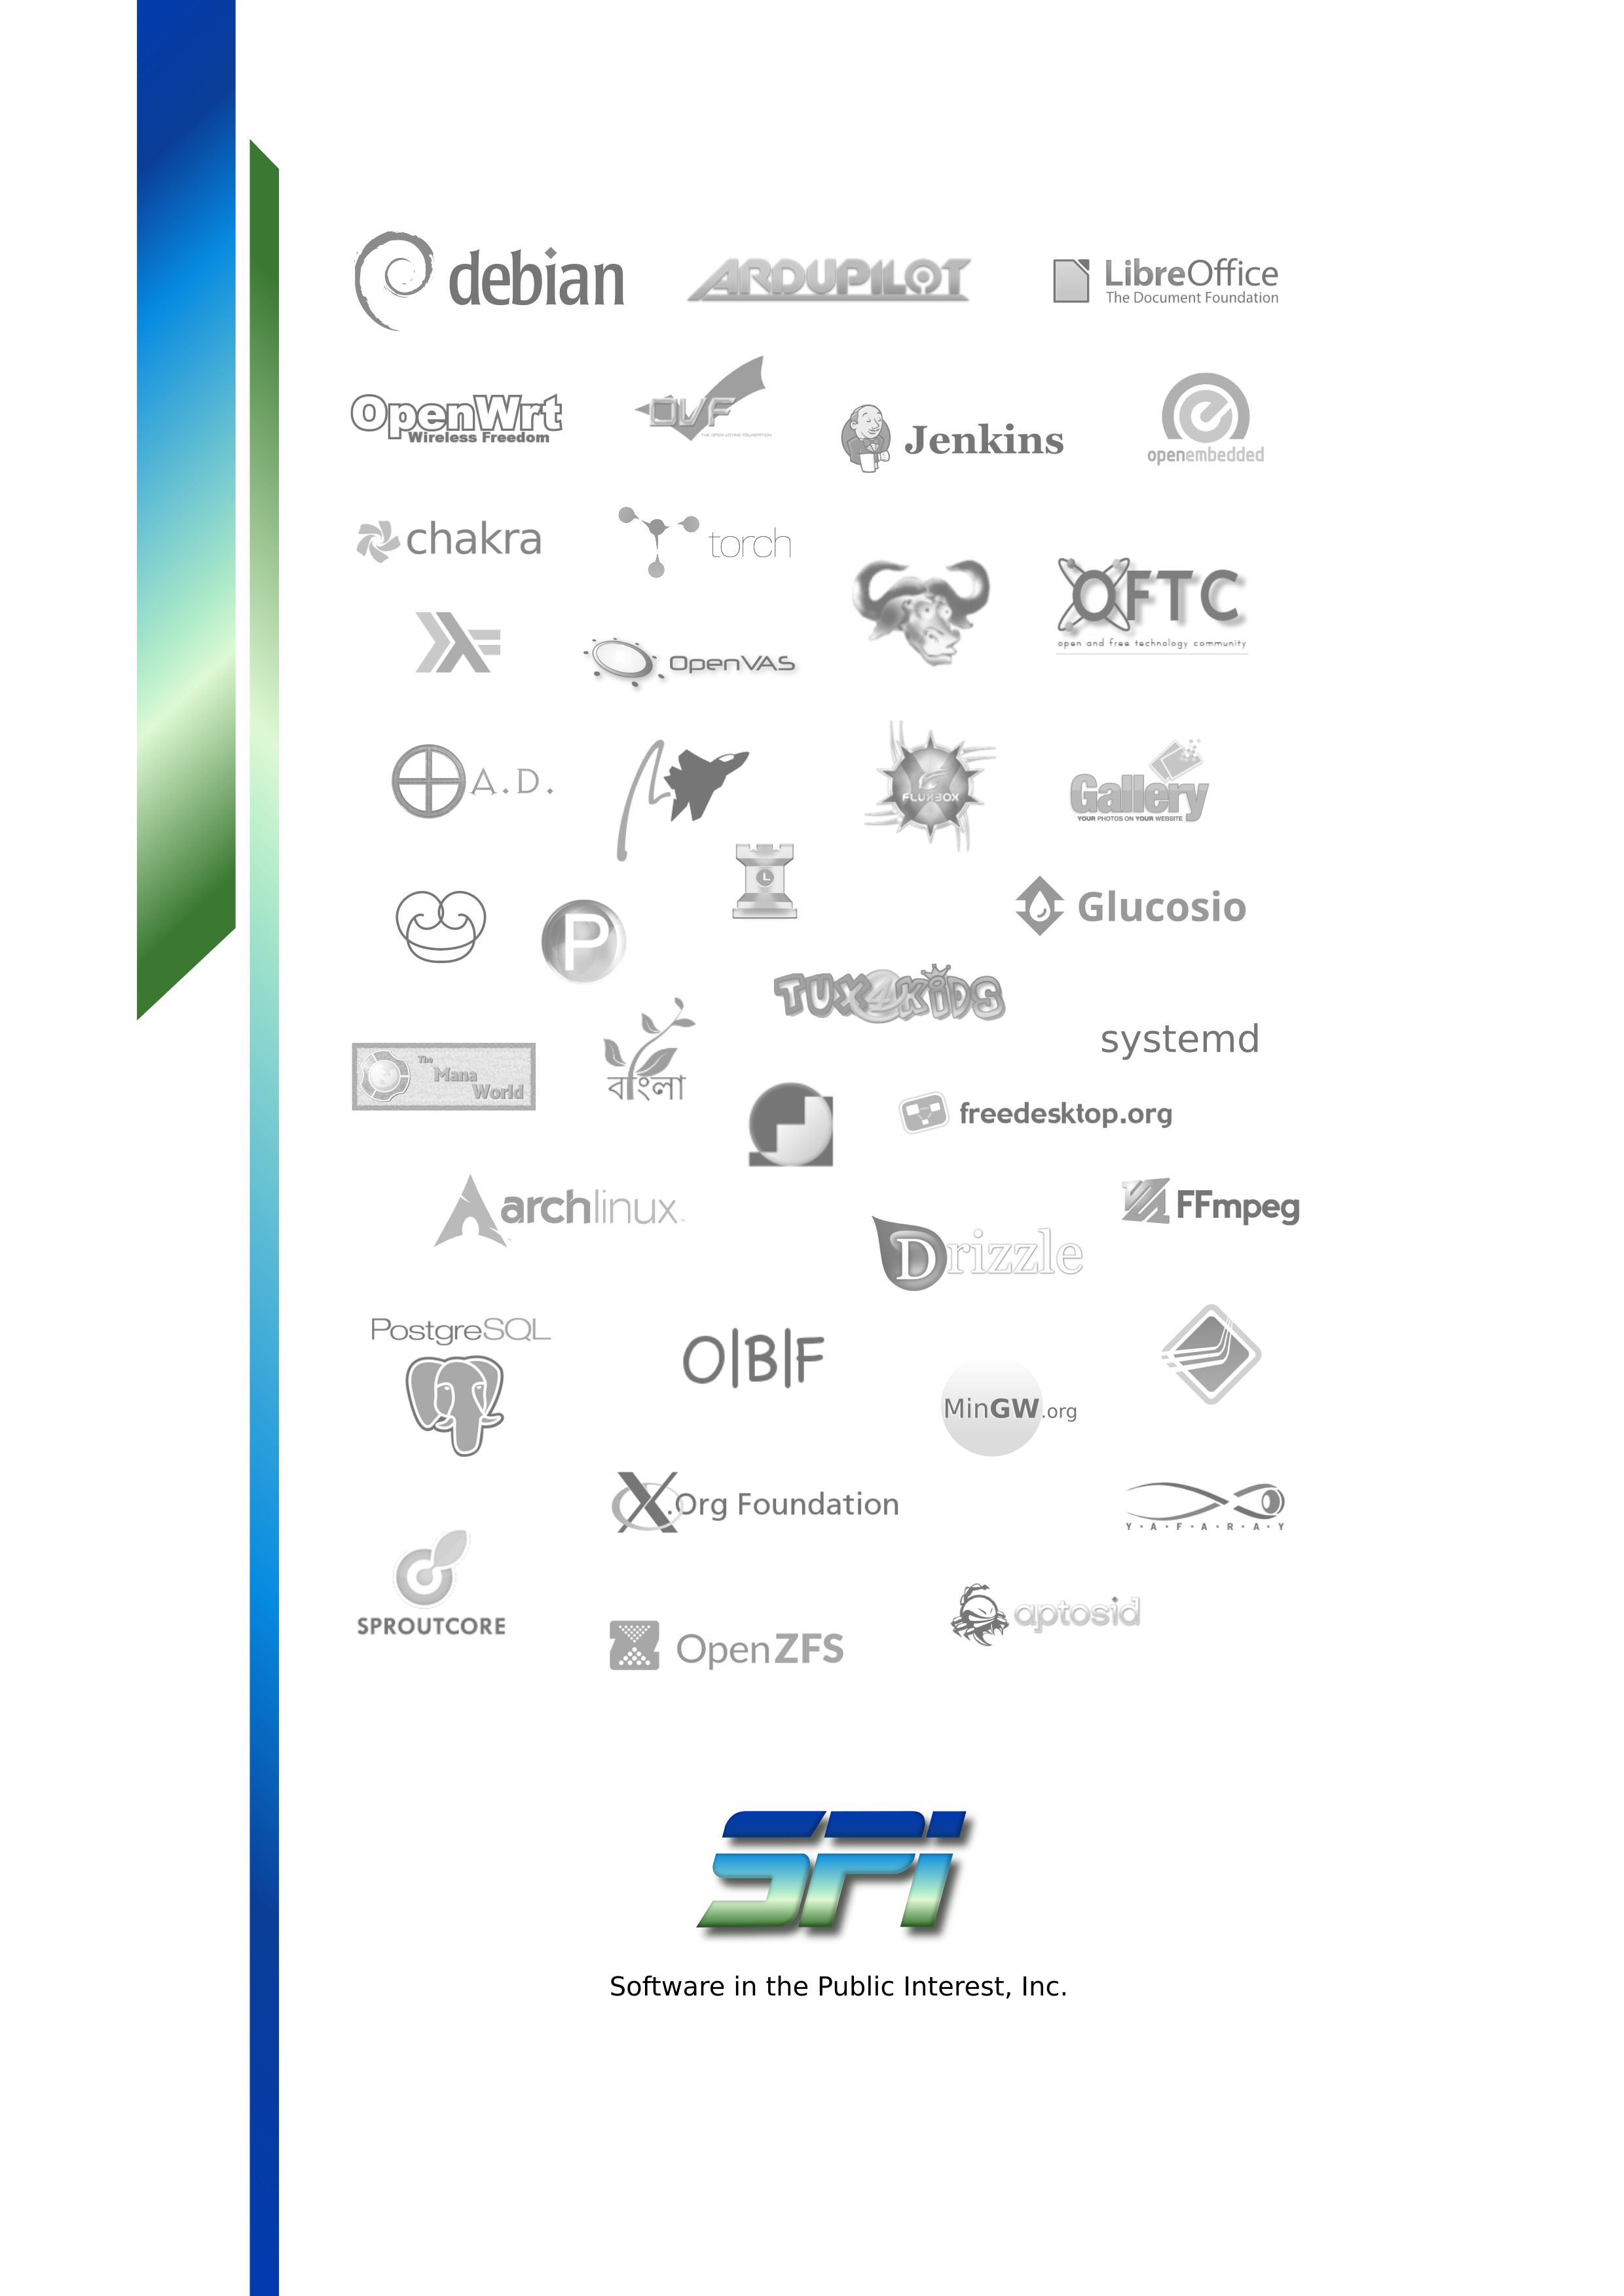
\includegraphics[width=\paperwidth,height=\paperheight]{images/spi-back-2018.jpg}}
}

\null

\end{document}
% Keep this at the bottom, thanks.
% Local Variables:
% TeX-master: "report"
% End:
